% =====================================================================
%  Introduction to Deep Learning — Class 15
%  Topic (course plan): Deep Networks
%  Subtopic (course plan): Normalization
%  Sources (course plan): Bishop Chapter 7, Prince Chapters 6-7
%
%  Classes 13 and 14 repaired the iteration.  This class repairs the
%  problem, so that the iteration has less to repair.  Order: the case
%  where one rescaling suffices, then depth defeating it, then training
%  defeating initialization, then small batches defeating batch
%  normalization.
%
%  Four results here are stated in neither textbook; the C variant is
%  this deck with those four removed.  See _shared/PLAN_Classes13_14_15.md.
%
%  Compile:  xelatex main.tex   (run twice)
% =====================================================================
\documentclass[aspectratio=169, 11pt]{beamer}

\usetheme{metropoliscustom}

\usepackage{graphicx}
\DeclareGraphicsExtensions{.pdf,.png,.jpg}
\graphicspath{{figs/}{Class15_Normalization/B_Recreated_Figures/figs/}}
\usepackage{amsmath, amssymb}
\usepackage{bm}
\usepackage{tikz}
\usetikzlibrary{arrows.meta, positioning, calc, decorations.pathreplacing,
                shapes.geometric, fit, backgrounds}
\tcbuselibrary{skins}

\definecolor{shc}{HTML}{341651}
\definecolor{tealc}{HTML}{1C7293}
\definecolor{dpc}{HTML}{800000}
\definecolor{accc}{HTML}{B8860B}

% ---- theorem environments -------------------------------------------
\setbeamertemplate{theorems}[numbered]
\usepackage{remreset}
\makeatletter\@removefromreset{theorem}{section}\makeatother
\renewcommand{\thetheorem}{\arabic{theorem}}
\newtheorem{lemmax}[theorem]{Lemma}
\newtheorem{propx}[theorem]{Proposition}
\newtheorem{corx}[theorem]{Corollary}
\newtheorem{algox}[theorem]{Algorithm}

% ---- parallel strip -------------------------------------------------
\newcommand{\twopar}[4]{%
  \vfill
  {\scriptsize
  \begin{tcolorbox}[enhanced, sidebyside, sidebyside align=top,
                    lefthand ratio=0.485,
                    segmentation style={shc!35, line width=0.6pt},
                    colback=shc!5, colframe=shc!35, boxrule=0.5pt,
                    arc=1.2mm, left=1.6mm, right=1.6mm,
                    top=0.6mm, bottom=0.6mm,
                    before skip=0pt, after skip=0pt]
    {\color{shc}\textbf{#1}}\hspace{0.55em}#2
  \tcblower
    {\color{dpc}\textbf{#3}}\hspace{0.55em}#4
  \end{tcolorbox}}%
  \vspace{0.35em}%
}

\newcommand{\bridge}[1]{%
  {\scriptsize\itshape\color{mcMuted} #1\par}\vspace{0.35em}}

\newcommand{\srcline}[1]{%
  \par\vspace{0.25em}%
  {\scriptsize\color{mcMuted}\hfill #1\par}}

\newcommand{\figsource}[1]{{\scriptsize\color{mcMuted} #1}}
\newcommand{\figcap}[2][0.90]{%
  \begin{center}\begin{minipage}{#1\textwidth}\centering
    {\scriptsize\color{mcMuted} #2}
  \end{minipage}\end{center}}

% =====================================================================
\title{Deep Networks}
\subtitle{Normalization}
\author{Introduction to Deep Learning \ \textperiodcentered\ Class 15}
\institute{}
\date{}

\footleft{Introduction to Deep Learning}
\footright{Normalization}
\titlelogos{}

\begin{document}

\maketitle

\begin{frame}{Outline}
  \tableofcontents
\end{frame}

% =====================================================================
\section{Where the Condition Number Comes From}
% =====================================================================

\begin{frame}{Repairing the problem instead of the iteration}
  \bridge{Class 14 spent its whole length working around a large
  condition number. It never asked where that number came from.}
  \vspace{0.35em}
  {\footnotesize
  \renewcommand{\arraystretch}{1.36}
  \begin{tabular}{@{}l@{\hspace{1.6em}}l@{}}
    \textbf{Classes 13 and 14} & \textbf{Today}\\
    change the \emph{step} & change the \emph{surface} the step is taken
      on\\
    momentum, schedules, Adam & rescale the inputs, the weights, the
      activations\\
    accept $\kappa$ and work around it & make $\kappa$ small in the
      first place\\
    one lever: the update rule & one lever: the parameterisation\\
  \end{tabular}}
  \vspace{0.9em}

  \begin{redhighlight}
    The condition number is not a fact of nature. It is a consequence of
    the units we happen to have measured things in, and of how the
    network is scaled.
  \end{redhighlight}
\end{frame}

\begin{frame}{Notation added today}
  \vspace{0.4em}
  {\footnotesize
  \renewcommand{\arraystretch}{1.34}
  \begin{columns}[T, onlytextwidth]
    \begin{column}{0.49\textwidth}
      \begin{tabular}{@{}l@{\hspace{1.5em}}l@{}}
        $\mu_i$, $\sigma_i^2$ & mean and variance of quantity $i$\\
        $\tilde{x}_{ni}$ & a normalized input\\
        $\hat{a}_{ni}$ & a normalized pre-activation\\
        $D$ & fan-in of a layer\\
      \end{tabular}
    \end{column}
    \begin{column}{0.49\textwidth}
      \begin{tabular}{@{}l@{\hspace{1.5em}}l@{}}
        $\sigma_w^2$ & variance of the initializer\\
        $\gamma_i$, $\beta_i$ & learnable scale and shift\\
        $K$ & mini-batch size in this class\\
        $M$ & units in a layer\\
      \end{tabular}
    \end{column}
  \end{columns}}
  \vspace{0.7em}

  \begin{itemize}\itemsep0.3em
    \item $\gamma$ and $\beta$ are learned by gradient descent alongside
          the weights, exactly like any other parameter
  \end{itemize}
\end{frame}

\begin{frame}{The Hessian of a linear model is a data matrix}
  \vspace{-0.25em}
  For $E(\mathbf{w}) = \sum_n (\mathbf{w}^{\mathsf T}\mathbf{x}_n - y_n)^2$ the curvature
  does not depend on $\mathbf{w}$ at all:
  \vspace{-0.35em}
  \[
    \mathbf{H} \;=\; 2\, \mathbf{X}^{\mathsf T} \mathbf{X} ,
    \qquad
    H_{ij} \;=\; 2 \sum_n x_{ni}\, x_{nj} .
  \]
  \vspace{-0.6em}
  \begin{itemize}\itemsep0.35em
    \item The diagonal $H_{ii}$ is the second moment of feature $i$: a
          feature measured on a large scale has large curvature
    \item The off-diagonal $H_{ij}$ is the correlation between features
          $i$ and $j$
    \item So $\kappa$ is a property of the \alert{data}, before any
          learning happens
  \end{itemize}
  \begin{redhighlight}
    Two things can wreck it: features on different \emph{scales}, and
    features that are \emph{correlated}. Only the first is easy to fix.
  \end{redhighlight}
\end{frame}

\begin{frame}{Two ways the data alone can wreck the conditioning}
  \begin{center}
    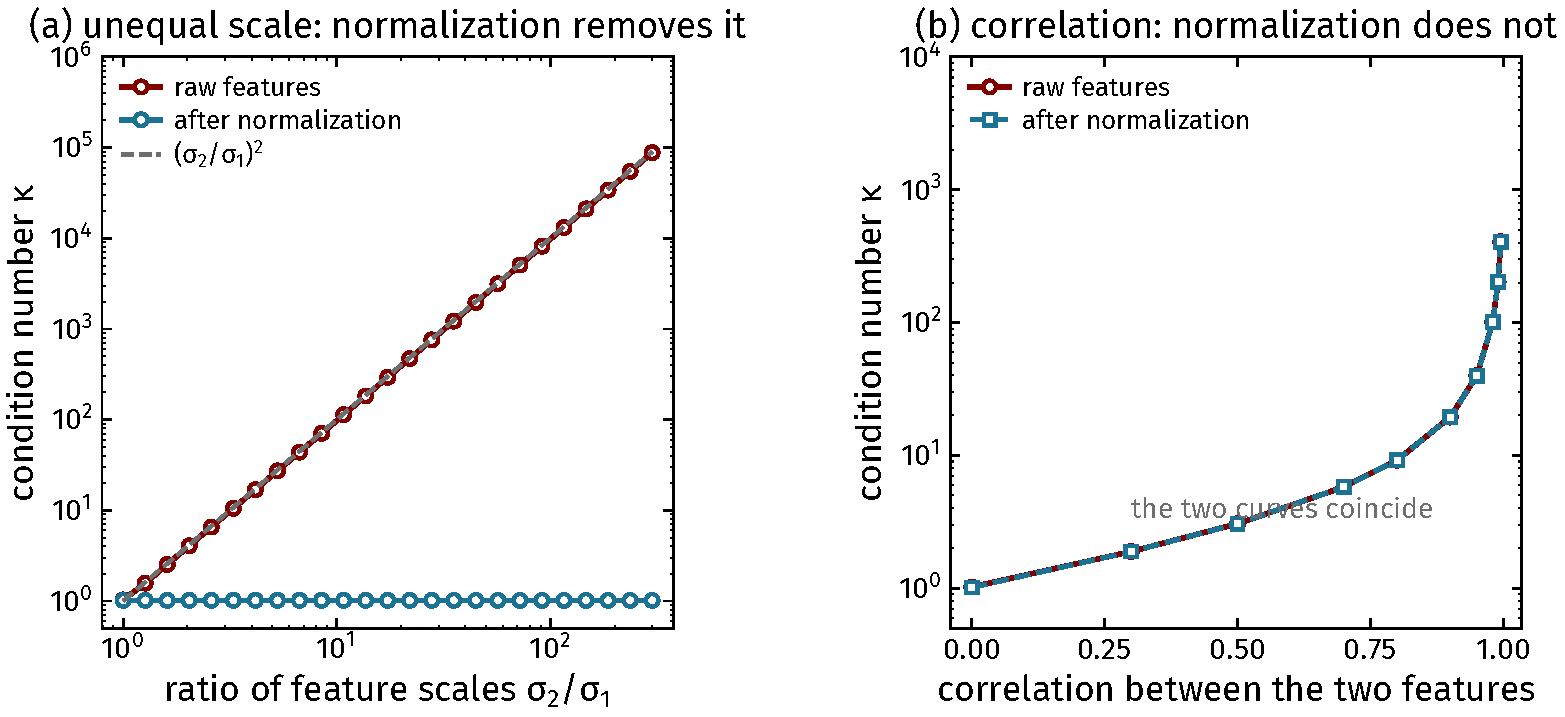
\includegraphics[height=0.52\textheight]{condition_from_data}
  \end{center}
  \figcap[0.97]{(a) two features of equal spread but different scale:
  $\kappa$ grows as the \emph{square} of the ratio, and per-feature
  rescaling removes it exactly. (b) two features of equal scale but
  correlated: $\kappa$ diverges, and rescaling does nothing.}
\end{frame}

\begin{frame}{The scale of a feature, squared}
  \vspace{-0.25em}
  \begin{propx}[Feature scale and the condition number]\label{th:scale}
    \small
    Let two uncorrelated, centred features have standard deviations
    $\sigma_1 \leq \sigma_2$. Then the least-squares Hessian
    $\mathbf{H} = 2\mathbf{X}^{\mathsf T}\mathbf{X}$ has
    $\kappa = (\sigma_2/\sigma_1)^{2}$, and after rescaling each feature
    to unit variance, $\kappa = 1$.
  \end{propx}
  \vspace{0.05em}
  {\footnotesize
  \begin{itemize}\itemsep0.26em
    \item \focus{1}{Uncorrelated and centred means $\sum_n x_{n1}x_{n2}
          \approx 0$, so $\mathbf{H}$ is diagonal.}
    \item \focus{2}{Its entries are $2N\sigma_1^2$ and $2N\sigma_2^2$,
          which are then its eigenvalues.}
    \item \focus{3}{Their ratio is $(\sigma_2/\sigma_1)^2$; dividing
          each feature by its own $\sigma$ makes both entries $2N$.
          \hfill $\square$}
  \end{itemize}}
  \vspace{-0.35em}
  \begin{redhighlight}
    Height in metres beside a platelet count in the hundreds of
    thousands gives $\kappa \sim 10^{10}$ before a weight is learned.
  \end{redhighlight}
\end{frame}

% =====================================================================
\section{Normalizing the Inputs}
% =====================================================================

\begin{frame}{Data normalization}
  \vspace{-0.5em}
  \begin{columns}[T, onlytextwidth]
    \begin{column}{0.47\textwidth}
      \[ \mu_i = \frac{1}{N}\sum_{n=1}^{N} x_{ni} \]
    \end{column}
    \begin{column}{0.50\textwidth}
      \[ \sigma_i^2 = \frac{1}{N}\sum_{n=1}^{N}(x_{ni} - \mu_i)^2 \]
    \end{column}
  \end{columns}
  \vspace{-0.6em}
  \[
    \tilde{x}_{ni} \;=\; \frac{x_{ni} - \mu_i}{\sigma_i}
  \]
  \vspace{-0.6em}
  \begin{itemize}\itemsep0.35em
    \item Every input now has zero mean and unit variance across the
          training set
    \item Computed \alert{once}, before training starts, because the
          inputs never change
    \item The \alert{same} $\mu_i$ and $\sigma_i$ must be applied to
          validation and test data
  \end{itemize}
  \srcline{Bishop \& Bishop (2024), Eqs.~7.48--7.50.}
\end{frame}

\begin{frame}{What that does to the error surface}
  \begin{center}
    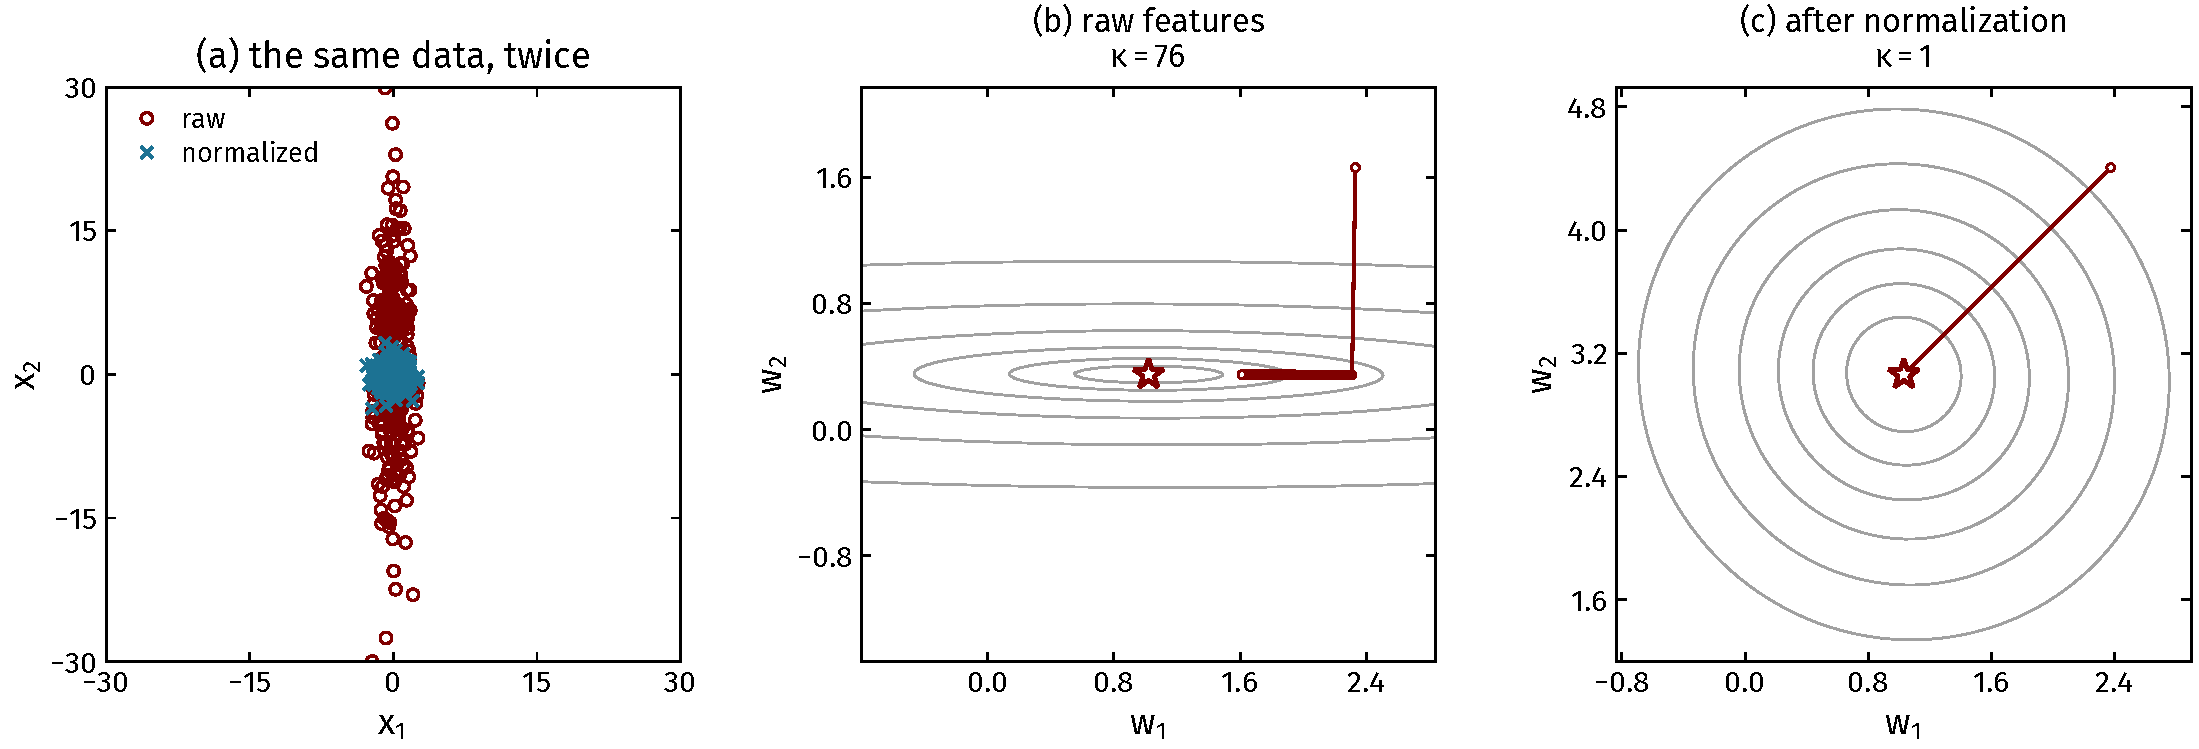
\includegraphics[width=0.93\linewidth]{input_scaling}
  \end{center}
  \figcap[0.98]{(a) the same points before and after rescaling. (b) the
  least-squares surface on the raw features, and gradient descent
  crawling along its floor. (c) the same surface after normalization:
  circular contours, and one step size that suits both directions.}
\end{frame}

\begin{frame}{What normalizing the inputs does not fix}
  \vspace{0.2em}
  \begin{itemize}\itemsep0.35em
    \item It fixes the \alert{diagonal} of $\mathbf{H}$; correlations live off
          the diagonal and survive untouched
    \item Removing those needs a rotation as well --- whitening ---
          which costs $O(d^3)$ and is rarely worth it
    \item A heavy-tailed feature can be normalized and still be
          dominated by a handful of points, so a transformation such as
          $\log$ often comes first
    \item Most importantly, it only touches the \alert{first} layer
  \end{itemize}
  \begin{redhighlight}
    Layer two sees the outputs of layer one, not the data. Nothing so
    far controls what those look like.
  \end{redhighlight}
\end{frame}

% =====================================================================
\section{Depth: Initialization}
% =====================================================================

\begin{frame}{What one layer does to the variance}
  \vspace{-0.25em}
  \begin{propx}[Variance across one ReLU layer]\label{th:var}
    \small
    Let $\mathbf{a}' = \mathbf{W} \mathbf{z}$ with $\mathbf{z} = \mathrm{ReLU}(\mathbf{a})$, the entries of $\mathbf{W}$ drawn
    independently from $\mathcal{N}(0, \sigma_w^2)$, the biases zero,
    and $\mathbf{a}$ symmetric about zero with variance $\sigma_a^2$. Then
    $\mathbb{E}[a'_i] = 0$ and
    \[
      \sigma_{a'}^2 \;=\; \tfrac12\, D\, \sigma_w^2\, \sigma_a^2 ,
    \]
    where $D$ is the fan-in of the layer.
  \end{propx}
  \vspace{0.05em}
  {\footnotesize
  \begin{itemize}\itemsep0.26em
    \item \focus{1}{$\mathbb{E}[a'_i] = \sum_j \mathbb{E}[w_{ij}]\,
          \mathbb{E}[z_j] = 0$, since $\mathbf{W}$ and $\mathbf{z}$ are independent and
          $\mathbf{W}$ has zero mean.}
    \item \focus{2}{So $\sigma_{a'}^2 = \mathbb{E}[a_i'^2]
          = \sigma_w^2 \sum_j \mathbb{E}[z_j^2]$.}
    \item \focus{3}{ReLU zeroes half of a symmetric distribution, giving
          $\mathbb{E}[z_j^2] = \tfrac12 \sigma_a^2$.}
    \item \focus{4}{Summing over the $D$ inputs gives the result.
          \hfill $\square$}
  \end{itemize}}
  \vspace{-0.4em}
  \srcline{Prince (2023), Eqs.~7.28--7.30; Bishop \& Bishop (2024),
  Eqs.~7.21--7.22.}
\end{frame}

\begin{frame}{One layer is a multiplication, so depth is a power}
  \vspace{-0.25em}
  \begin{corx}[Geometric growth or geometric decay]\label{th:geom}
    \small
    Applying Proposition~\ref{th:var} $K$ times,
    \[
      \sigma^2_{a^{(K)}} \;=\;
        \left(\tfrac12 D \sigma_w^2\right)^{K} \sigma^2_{a^{(0)}} .
    \]
    The variance therefore explodes if
    $\tfrac12 D \sigma_w^2 > 1$, vanishes if it is less than one, and is
    preserved only when it equals one exactly.
  \end{corx}
  \vspace{0.25em}
  \begin{itemize}\itemsep0.3em
    \item There is no safe margin: any factor other than one, raised to
          the fiftieth power, is a catastrophe
    \item $D = 100$ with $\sigma_w^2 = 0.1$ gives a factor of $5$, so
          fifty layers multiply the variance by $5^{50} \approx 10^{35}$
  \end{itemize}
\end{frame}

\begin{frame}{Fifty layers, five initializations}
  \begin{center}
    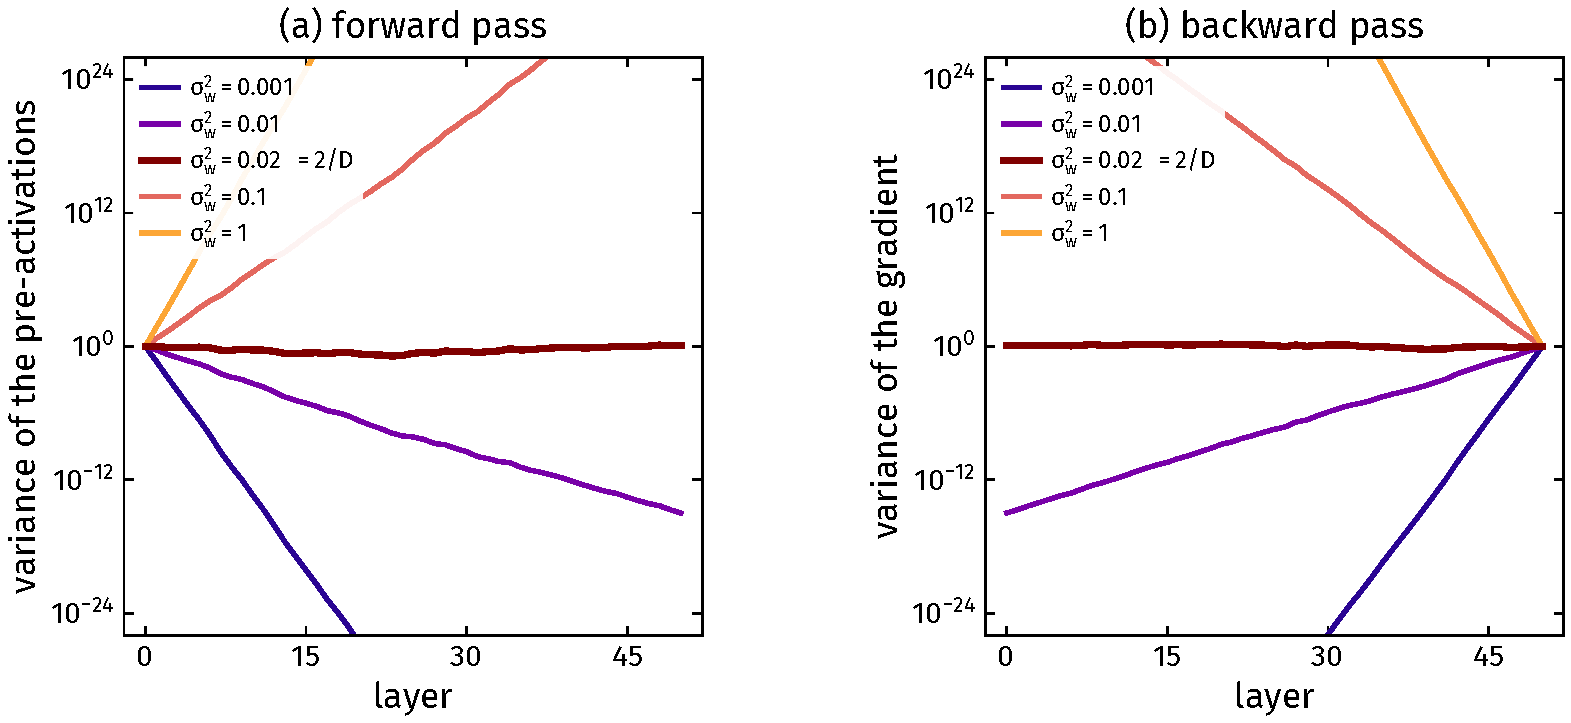
\includegraphics[height=0.52\textheight]{variance_depth}
  \end{center}
  \figcap[0.97]{Fifty layers of one hundred units. (a) the variance of
  the pre-activations going forward. (b) the variance of the gradient
  coming back. Only one value of $\sigma_w^2$ stays level, and it is the
  one that makes the factor exactly one.}
\end{frame}

\begin{frame}{The same problem, seen through the chain rule}
  \vspace{-0.35em}
  \[
    \frac{\partial E}{\partial w_i}
      = \sum_m \cdots \sum_l \sum_j
        \frac{\partial z^{(1)}_m}{\partial w_i} \cdots
        \frac{\partial z^{(K)}_j}{\partial z^{(K-1)}_l}
        \frac{\partial E}{\partial z^{(K)}_j}
  \]
  \vspace{-0.7em}
  \begin{itemize}\itemsep0.3em
    \item A gradient in the first layer is a product of $K$ Jacobians:
          if most factors are below one it tends to zero, and above one
          to infinity
    \item These are the \alert{vanishing} and \alert{exploding} gradient
          problems, met in Class 11 as a property of the activation
          function and appearing here as a property of \emph{scale}
    \item Matching the variance forward needs $\sigma_w^2 = 2/D$;
          backward it needs $2/D'$, with $D'$ the fan-out
  \end{itemize}
  \srcline{Bishop \& Bishop (2024), Eq.~7.51; Prince (2023), Eq.~7.32.}
\end{frame}

\begin{frame}{He initialization}
  \vspace{-0.3em}
  \begin{propx}[The variance that preserves scale]\label{th:he}
    \small
    Setting $\tfrac12 D \sigma_w^2 = 1$, that is
    \[
      \sigma_w^2 \;=\; \frac{2}{D},
      \qquad\text{equivalently}\qquad
      \sigma_w \;=\; \sqrt{\frac{2}{D}} ,
    \]
    makes the variance of the pre-activations the same in every layer.
  \end{propx}
  \vspace{0.25em}
  \begin{itemize}\itemsep0.3em
    \item The factor of two is exactly the half of the distribution that
          ReLU discards; without ReLU the rule is $1/D$
    \item Drawn from $\mathcal{N}(0, \sigma_w^2)$, or a uniform
          distribution with the same variance; the rule is per layer, so
          more inputs means smaller weights
  \end{itemize}
  \srcline{He et al.~(2015); Bishop \& Bishop (2024), Eq.~7.23;
  Prince (2023), Eq.~7.31.}
\end{frame}

\begin{frame}{When the layer is not square}
  \vspace{-0.35em}
  \[
    \underbrace{\sigma_w^2 = \frac{2}{D}}_{\text{forward}}
    \qquad
    \underbrace{\sigma_w^2 = \frac{2}{D'}}_{\text{backward}}
    \qquad
    \underbrace{\sigma_w^2 = \frac{4}{D + D'}}_{\text{the compromise}}
  \]
  \vspace{-0.65em}
  \begin{itemize}\itemsep0.3em
    \item If $D \neq D'$ the two conditions cannot both hold, so an
          average of the two is used
    \item This is \alert{Glorot} initialization; it predates He and
          omits the factor of two, having been derived for sigmoidal
          units
    \item Biases start at zero, or at a small positive value for ReLU so
          that most units are active and passing gradient
  \end{itemize}
  \srcline{Glorot \& Bengio (2010); Prince (2023), Eq.~7.33.}
\end{frame}

\begin{frame}{The three rules, and what they do at depth}
  \begin{center}
    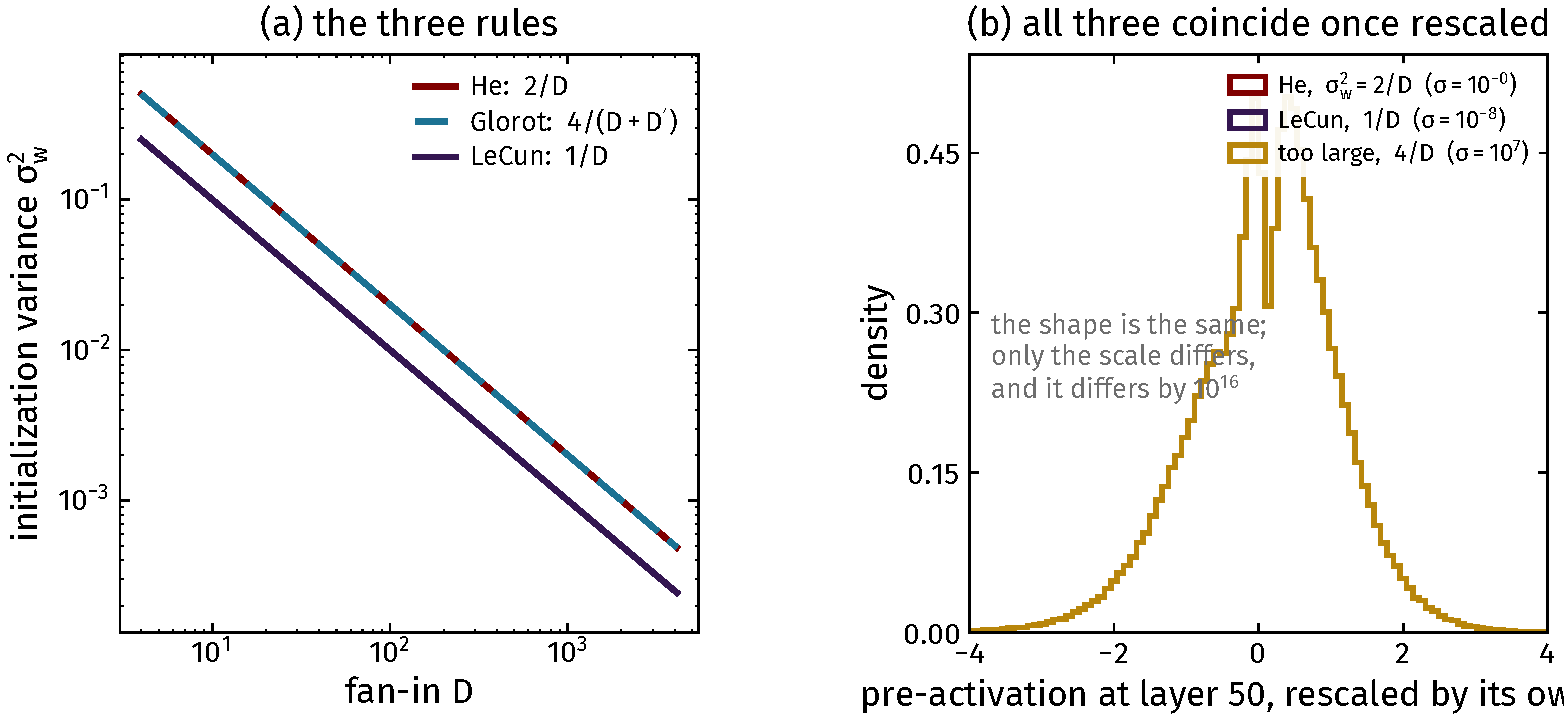
\includegraphics[height=0.52\textheight]{init_rules}
  \end{center}
  \figcap[0.97]{(a) the prescribed variance against the fan-in. (b) the
  distribution of pre-activations at layer fifty under three rules,
  each rescaled by its own standard deviation: the shape is identical
  and only the scale differs --- by sixteen orders of magnitude.}
\end{frame}

\begin{frame}{Why the weights cannot all start equal}
  \vspace{-0.35em}
  \begin{propx}[Symmetry is never broken by gradient descent]\label{th:sym}
    \small
    Two hidden units that receive the same inputs and are initialized
    with identical incoming and outgoing weights compute the same
    function, receive the same gradient, and remain identical after
    every update.
  \end{propx}
  {\footnotesize
  \begin{itemize}\itemsep0.28em
    \item \focus{1}{Identical incoming weights and inputs give identical
          pre-activations, hence identical activations.}
    \item \focus{2}{Identical outgoing weights give both the same
          $\partial E / \partial z_j$.}
    \item \focus{3}{Each weight gradient is that quantity times the same
          input, so the updates coincide, and by induction they stay
          identical. \hfill $\square$}
  \end{itemize}}
  \vspace{-0.3em}
  \srcline{Bishop \& Bishop (2024), \S7.2.5.}
\end{frame}

\begin{frame}{Symmetry, drawn}
  \begin{center}
    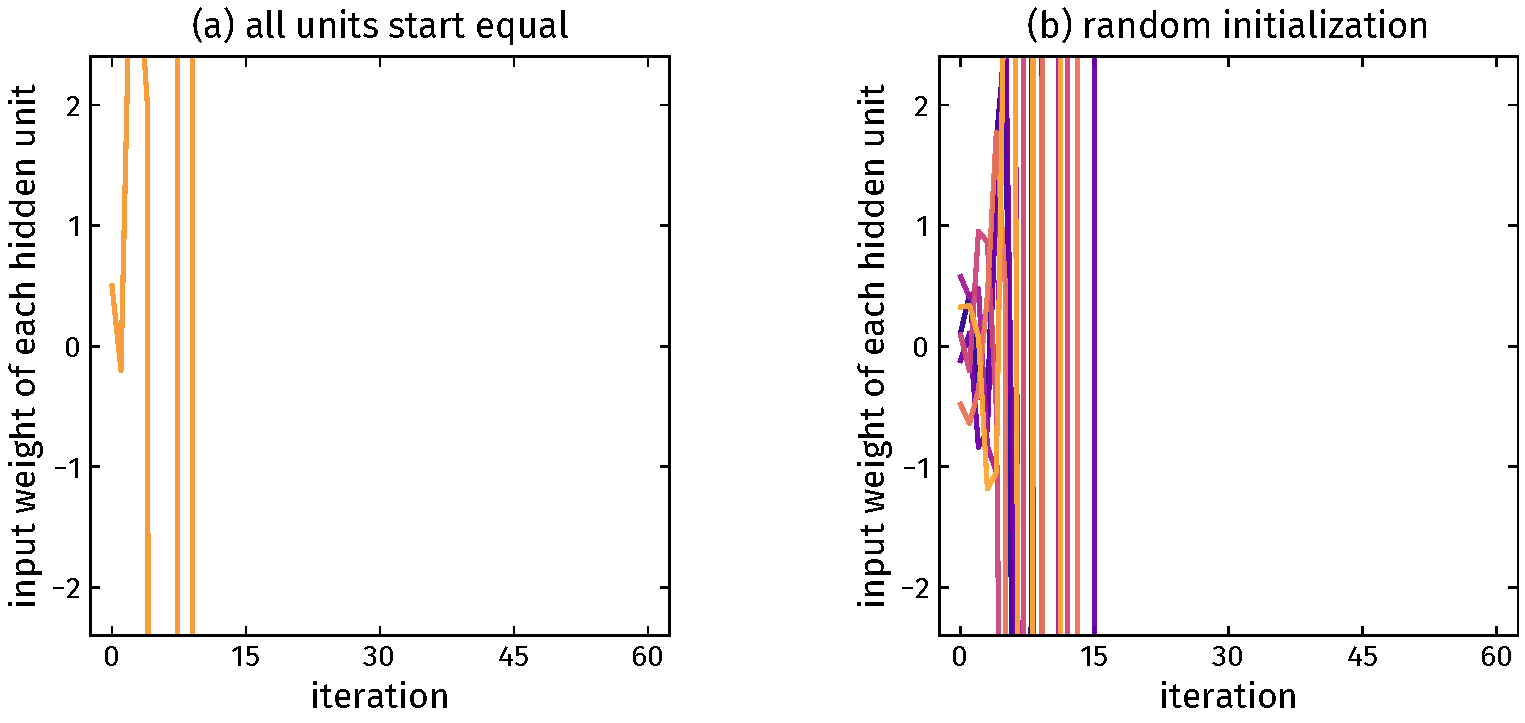
\includegraphics[height=0.52\textheight]{symmetry}
  \end{center}
  \figcap[0.97]{Six hidden units fitting the same target. (a) started
  identically, they trace one curve and stay on it, so the layer has the
  capacity of a single unit. (b) started from random values, they
  separate and specialise. Random initialization is what makes a wide
  layer wide.}
\end{frame}

% =====================================================================
\section{Training: Batch Normalization}
% =====================================================================

\begin{frame}{Initialization is a statement about the first step}
  \bridge{The weights are chosen so that every layer starts at unit
  variance. Then training changes the weights.}
  \vspace{0.4em}
  \begin{itemize}\itemsep0.42em
    \item Nothing in the argument of the last section survives the first
          update, because it was an argument about a particular
          distribution of weights
    \item After a few hundred steps the deeper layers are nowhere near
          where they were placed
    \item The deeper the network, the sooner and the worse the drift
    \item The same reasoning that motivated normalizing the inputs
          applies to \emph{every} layer --- with one difference: it must
          be redone continuously
  \end{itemize}
  \srcline{Bishop \& Bishop (2024), \S7.4.2.}
\end{frame}

\begin{frame}{The statistics do not stay where they were put}
  \begin{center}
    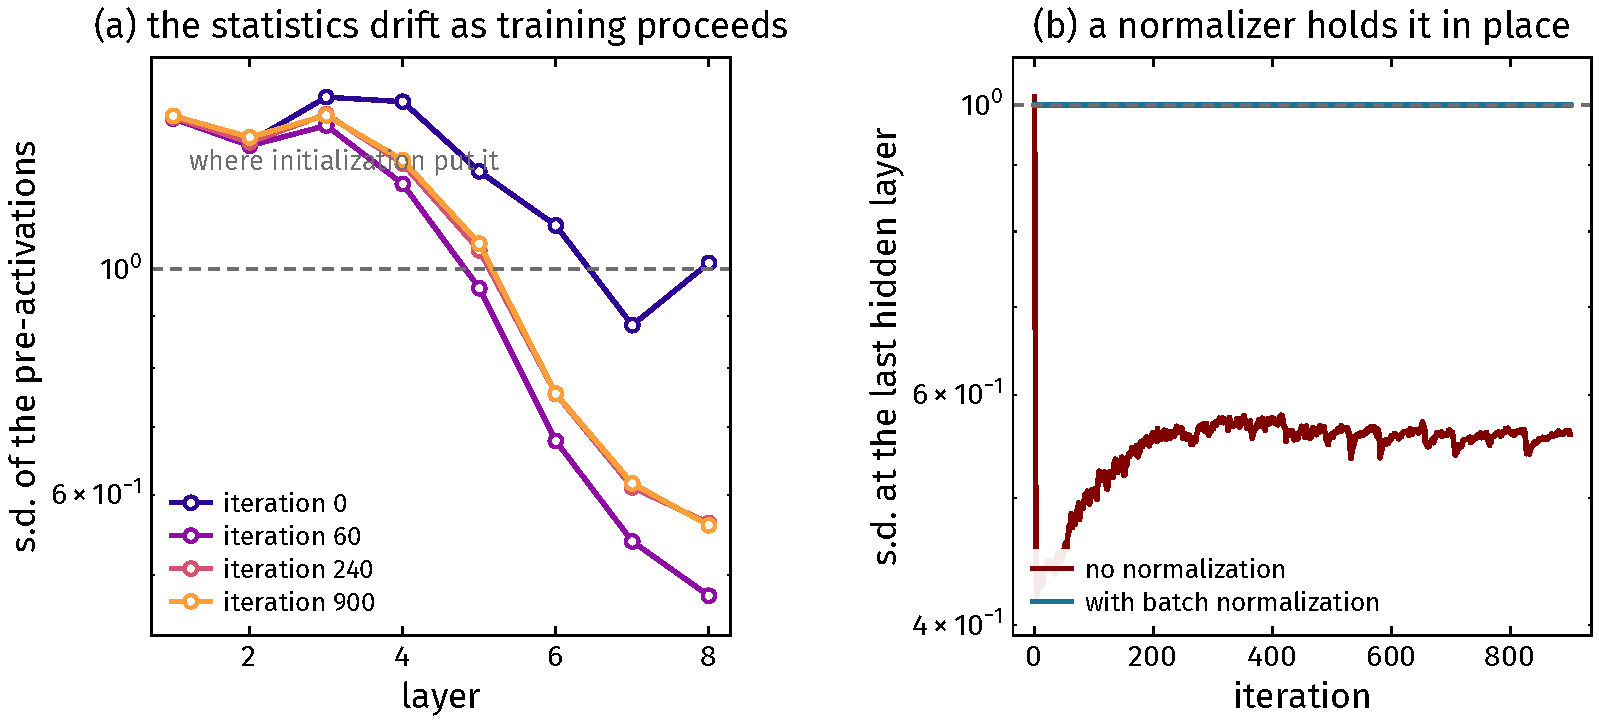
\includegraphics[height=0.52\textheight]{drift}
  \end{center}
  \figcap[0.97]{An eight-layer network initialized so that every layer
  starts at unit variance. (a) the spread of the pre-activations by
  layer, at four points during training. (b) the same quantity at the
  last hidden layer, against the iteration.}
\end{frame}

\begin{frame}{Batch normalization}
  \vspace{-0.55em}
  \begin{columns}[T, onlytextwidth]
    \begin{column}{0.47\textwidth}
      \[ \mu_i = \frac{1}{K}\sum_{n=1}^{K} a_{ni} \]
    \end{column}
    \begin{column}{0.50\textwidth}
      \[ \sigma_i^2 = \frac{1}{K}\sum_{n=1}^{K}(a_{ni} - \mu_i)^2 \]
    \end{column}
  \end{columns}
  \vspace{-0.6em}
  \[
    \hat{a}_{ni} \;=\; \frac{a_{ni} - \mu_i}{\sqrt{\sigma_i^2 +
      \varepsilon}}
  \]
  \vspace{-0.7em}
  \begin{itemize}\itemsep0.28em
    \item The sums run over the $K$ members of the \alert{mini-batch},
          separately for each hidden unit $i$
    \item Exactly the input-normalization formula, applied to a hidden
          layer and recomputed at every step
    \item Either the pre-activations or the activations may be
          normalized
  \end{itemize}
  \srcline{Ioffe \& Szegedy (2015); Bishop \& Bishop (2024),
  Eqs.~7.52--7.54.}
\end{frame}

\begin{frame}{Giving the scale back, on purpose}
  \vspace{-0.35em}
  \[
    \tilde{a}_{ni} \;=\; \gamma_i\, \hat{a}_{ni} + \beta_i
  \]
  \vspace{-0.85em}
  \begin{itemize}\itemsep0.26em
    \item Forcing zero mean and unit variance removes degrees of
          freedom, so two learnable parameters per unit hand them back
    \item It looks as though this undoes the normalization: the mean and
          variance can be anything again
    \item The difference is \alert{how they are reached}: before, a
          complicated function of every weight below; now, two
          parameters set directly
  \end{itemize}
  \srcline{Bishop \& Bishop (2024), Eq.~7.55.}
\end{frame}

\begin{frame}{Which entries share a mean}
  \begin{center}
    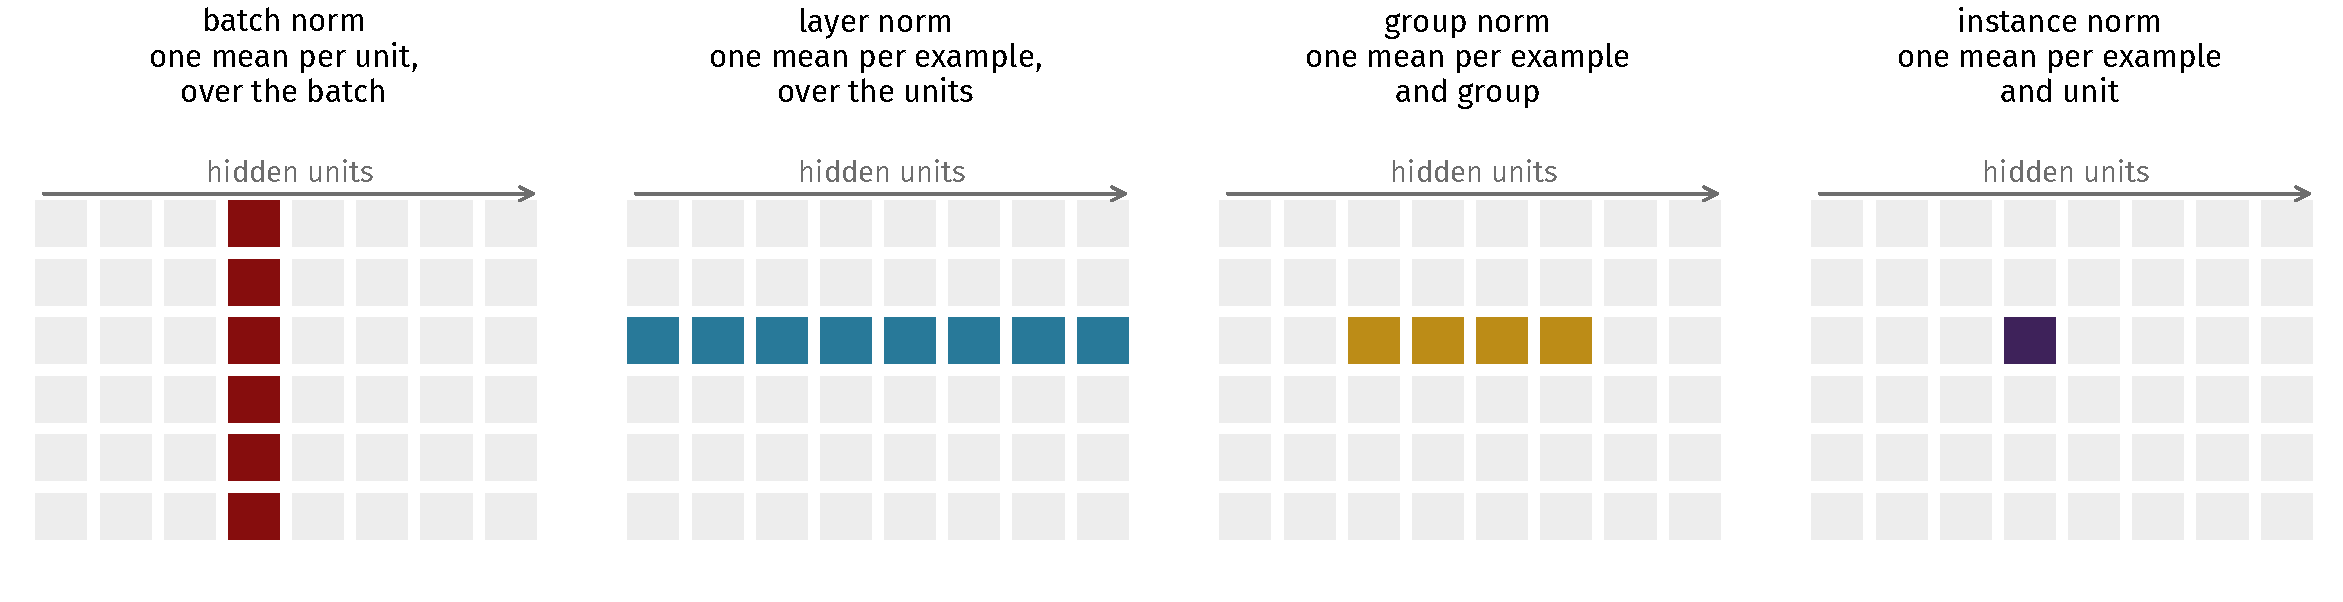
\includegraphics[width=0.95\linewidth]{norm_axes}
  \end{center}
  \figcap[0.98]{Rows are the members of a mini-batch and columns are the
  hidden units. The shaded cells are pooled to produce one mean and one
  variance. Every normalizer in this class is this picture with a
  different set of cells shaded.}
\end{frame}

\begin{frame}{Training time and inference time differ}
  \vspace{-0.35em}
  \[
    \bar\mu_i^{(\tau)} = \alpha\,\bar\mu_i^{(\tau-1)}
      + (1-\alpha)\,\mu_i,
    \qquad
    \bar\sigma_i^{(\tau)} = \alpha\,\bar\sigma_i^{(\tau-1)}
      + (1-\alpha)\,\sigma_i
  \]
  \vspace{-0.9em}
  \begin{itemize}\itemsep0.26em
    \item At prediction time there is no mini-batch: a single example
          has no variance of its own
    \item Evaluating them over the training set afterwards would work,
          and is too expensive, so running averages are accumulated
          \emph{during} training and used at inference
    \item The network therefore computes a slightly different function
          in the two phases \hfill \figsource{B\&B (2024),
          Eqs.~7.56--7.57}
  \end{itemize}
\end{frame}

\begin{frame}{What it buys}
  \begin{center}
    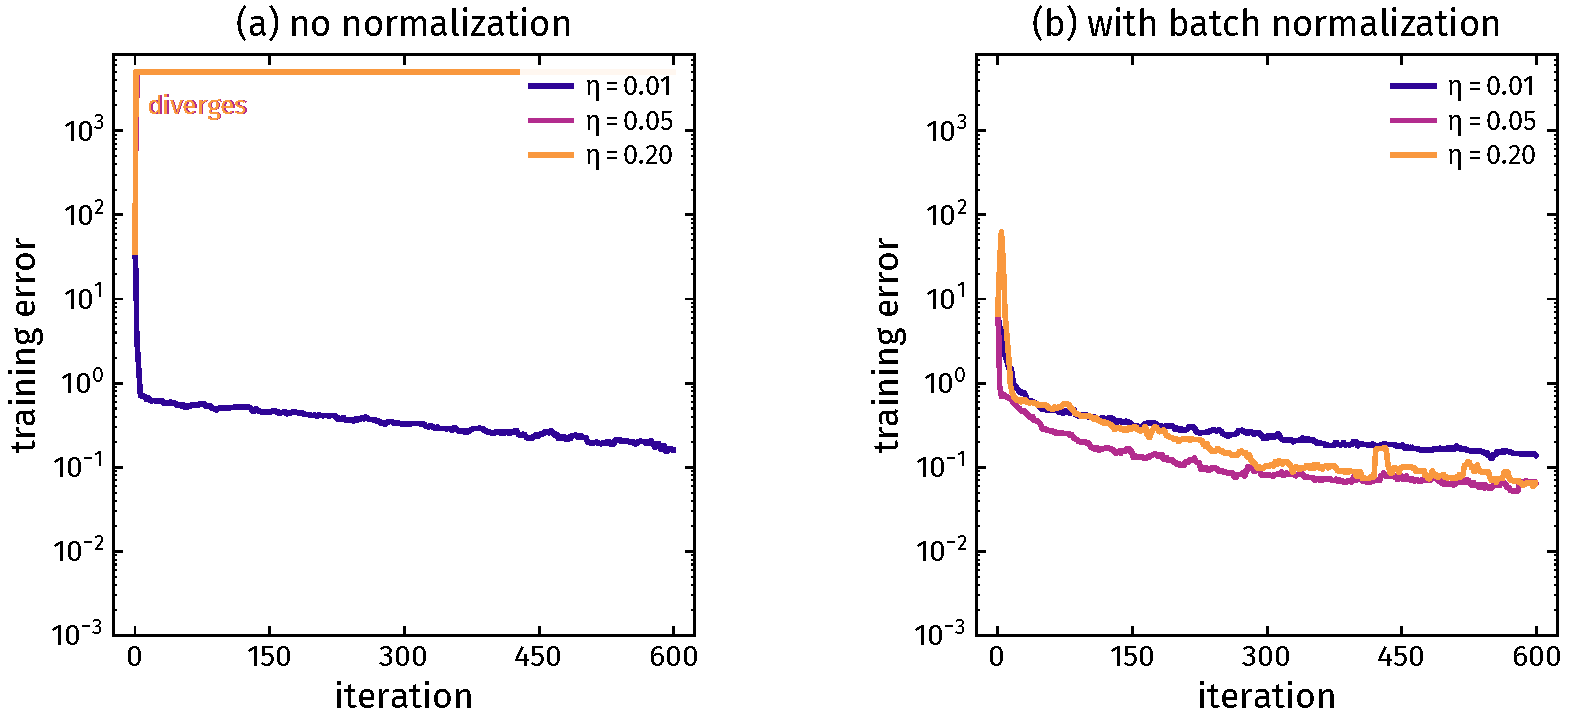
\includegraphics[height=0.52\textheight]{bn_effect}
  \end{center}
  \figcap[0.97]{The same network, data and initialization at three
  learning rates. (a) without normalization only the smallest is
  stable. (b) with batch normalization all three are stable, and the
  largest is now the fastest.}
\end{frame}

\begin{frame}{A normalized layer does not care how big its weights are}
  \vspace{-0.25em}
  \begin{propx}[Scale invariance]\label{th:scaleinv}
    \small
    Let a layer's pre-activations be normalized. Multiplying every
    weight feeding into it by $a > 0$ leaves the layer's output
    unchanged, and scales the gradient with respect to those weights by
    $1/a$.
  \end{propx}
  \vspace{0.05em}
  {\footnotesize
  \begin{itemize}\itemsep0.26em
    \item \focus{1}{Scaling $\mathbf{W}$ by $a$ scales the pre-activations, their
          mean and their standard deviation all by $a$.}
    \item \focus{2}{The ratio $(a - \mu)/\sigma$ is therefore unchanged,
          so $E(a\mathbf{W}) = E(\mathbf{W})$ for every $a$.}
    \item \focus{3}{Differentiating in $\mathbf{W}$ gives
          $a\,\nabla E(aW) = \nabla E(W)$. \hfill $\square$}
  \end{itemize}}
  \vspace{-0.7em}
  \begin{redhighlight}
    A layer whose weights have grown takes smaller steps: a per-layer
    learning rate nobody had to tune.
  \end{redhighlight}
\end{frame}

\begin{frame}{Scale invariance, measured}
  \begin{center}
    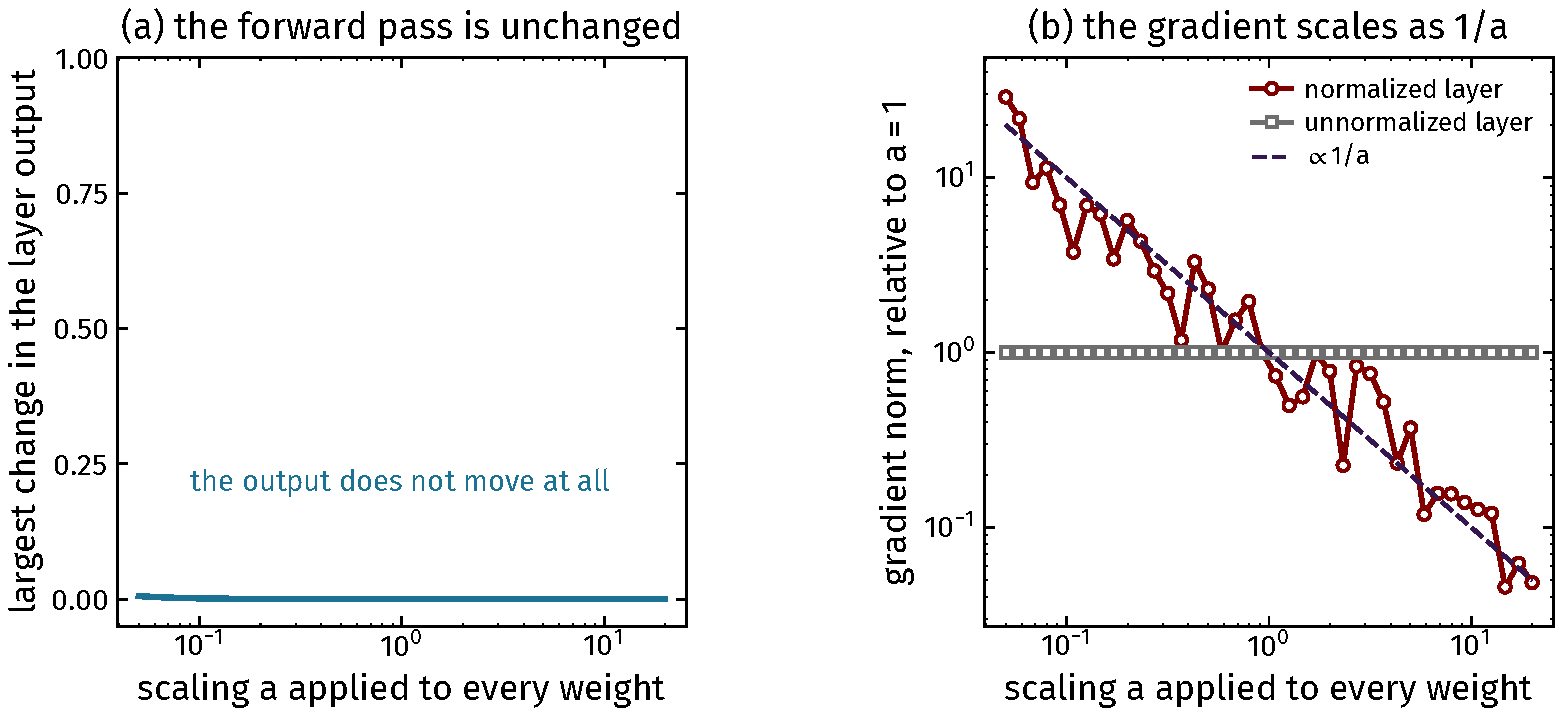
\includegraphics[height=0.52\textheight]{scale_invariance}
  \end{center}
  \figcap[0.97]{(a) the output of a normalized layer as every incoming
  weight is scaled over three orders of magnitude. (b) the norm of the
  gradient with respect to those weights, relative to its value at
  $a=1$, against the $1/a$ law.}
\end{frame}

\begin{frame}{Why it works is not what was first claimed}
  \vspace{0.3em}
  \begin{itemize}\itemsep0.42em
    \item The original argument was \alert{internal covariate shift}:
          updating early layers changes the distribution that later
          layers see, and normalizing removes that
    \item Later work found covariate shift is not the significant
          factor. Deliberately injecting distribution shift after a
          normalization layer does not undo the benefit
    \item What does change is the \alert{smoothness} of the error
          surface: with normalization, the error and the gradient vary
          far less over the distance of one step
    \item A gradient that predicts the next gradient well is a gradient
          you can take a large step along --- which is exactly what
          Class 14 was short of
  \end{itemize}
  \srcline{Santurkar et al.~(2018); Bishop \& Bishop (2024), \S7.4.2.}
\end{frame}

\begin{frame}{Smoothness, measured}
  \begin{center}
    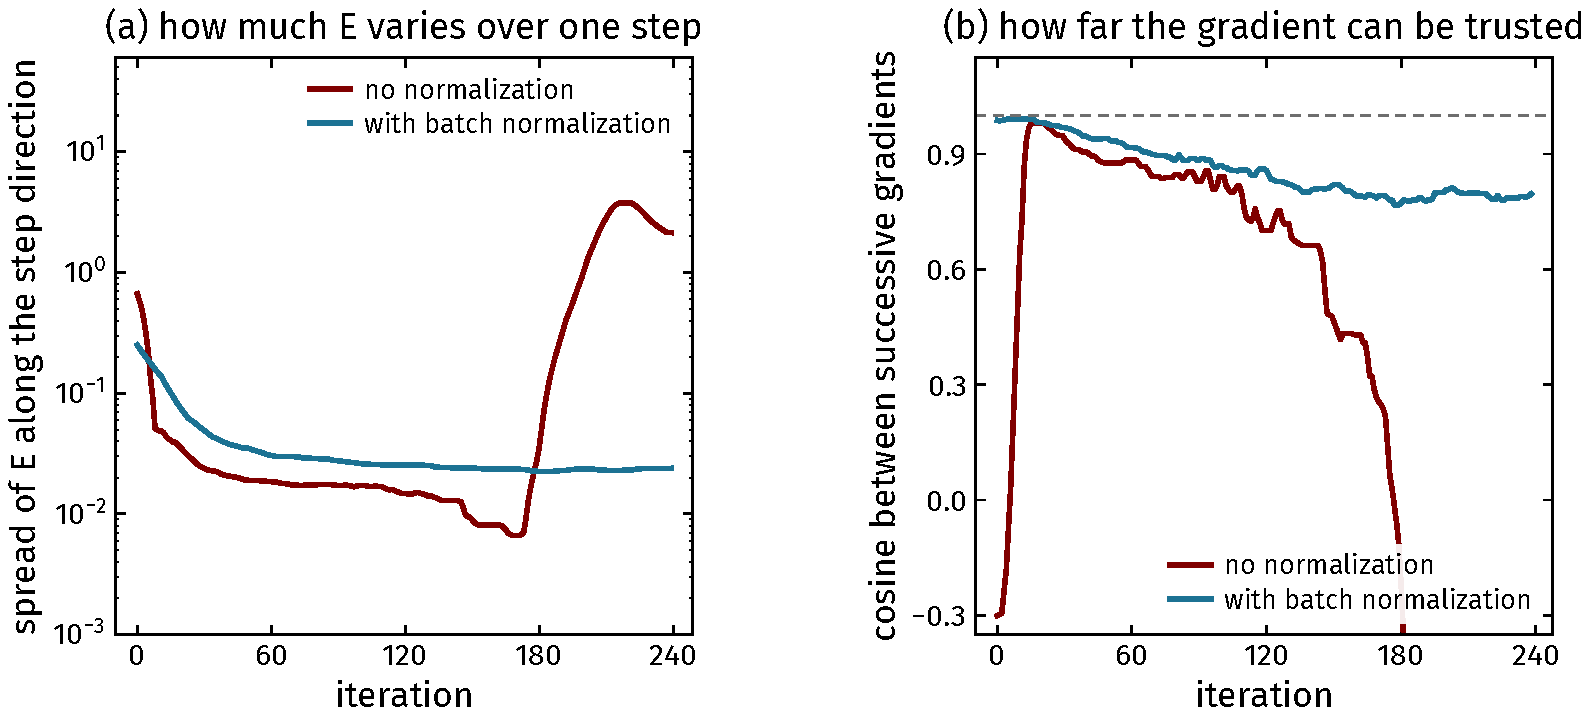
\includegraphics[height=0.52\textheight]{smoothness}
  \end{center}
  \figcap[0.97]{(a) how much the error varies along the descent
  direction over one step. (b) the cosine between successive gradients:
  how far the direction measured here still points the right way one
  step later.}
\end{frame}

% =====================================================================
\section{Small Batches: Layer Normalization}
% =====================================================================

\begin{frame}{Three places batch normalization breaks}
  \vspace{0.25em}
  \begin{itemize}\itemsep0.38em
    \item \alert{Small batches.} The statistics are estimates from $K$
          samples, with standard error $\propto 1/\sqrt{K}$; below a few
          dozen the correction is mostly noise
    \item \alert{Distributed training.} The batch is split across
          devices, and pooling across them costs a synchronisation at
          every layer
    \item \alert{Sequences.} In a recurrent network the distribution
          changes at every time step, so there is no fixed population
  \end{itemize}
  \vspace{0.4em}
  \begin{redhighlight}
    All three have the same cause: the statistics are taken across the
    \emph{batch}. Take them across the \emph{units} instead and all
    three disappear.
  \end{redhighlight}
  \srcline{Bishop \& Bishop (2024), \S7.4.3.}
\end{frame}

\begin{frame}{The batch size the statistics depend on}
  \begin{center}
    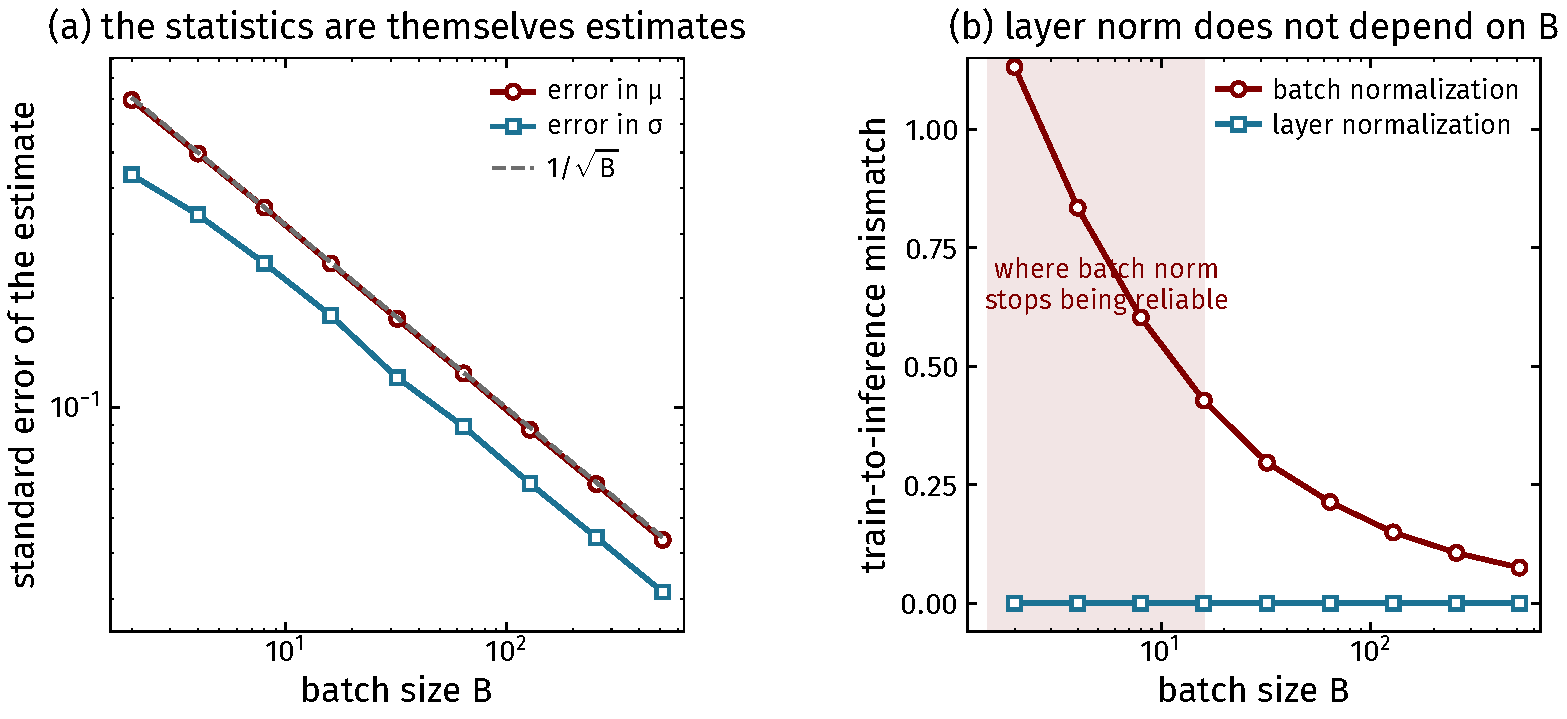
\includegraphics[height=0.52\textheight]{bn_batchsize}
  \end{center}
  \figcap[0.97]{(a) the standard error of the estimated mean and
  standard deviation against the batch size. (b) the resulting mismatch
  between what is used in training and what is used at inference; layer
  normalization uses no batch statistics and is flat.}
\end{frame}

\begin{frame}{Layer normalization}
  \vspace{-0.55em}
  \begin{columns}[T, onlytextwidth]
    \begin{column}{0.47\textwidth}
      \[ \mu_n = \frac{1}{M}\sum_{i=1}^{M} a_{ni} \]
    \end{column}
    \begin{column}{0.50\textwidth}
      \[ \sigma_n^2 = \frac{1}{M}\sum_{i=1}^{M}(a_{ni} - \mu_n)^2 \]
    \end{column}
  \end{columns}
  \vspace{-0.6em}
  \[
    \hat{a}_{ni} \;=\; \frac{a_{ni} - \mu_n}{\sqrt{\sigma_n^2 +
      \varepsilon}}
  \]
  \vspace{-0.7em}
  \begin{itemize}\itemsep0.28em
    \item The identical expression with the sum over the $M$
          \alert{units} instead of the $K$ examples, and the same
          learnable $\gamma_i$, $\beta_i$
    \item Each example is normalized on its own, so training and
          inference compute the \alert{same} function and no running
          averages are needed
    \item Introduced for recurrent networks; now standard in
          transformers
  \end{itemize}
  \srcline{Ba, Kiros \& Hinton (2016); Bishop \& Bishop (2024),
  Eqs.~7.58--7.60.}
\end{frame}

\begin{frame}{Four normalizers, one formula}
  \vspace{0.3em}
  {\footnotesize
  \renewcommand{\arraystretch}{1.42}
  \begin{tabular}{@{}l@{\hspace{1.3em}}l@{\hspace{1.3em}}l@{}}
    \textbf{Method} & \textbf{Average taken over} & \textbf{Used when}\\
    batch norm & the batch, per unit & convolutional vision, large
      batches\\
    layer norm & the units, per example & transformers, recurrent
      networks\\
    group norm & a block of units, per example & vision with small
      batches\\
    instance norm & one unit, per example & style transfer, image
      generation\\
  \end{tabular}}
  \vspace{0.6em}

  \begin{itemize}\itemsep0.28em
    \item All four subtract a mean, divide by a standard deviation, then
          apply a learnable $\gamma$ and $\beta$; they differ
          \alert{only} in which entries are pooled
    \item Group norm interpolates: one group is layer norm, and as many
          groups as units is instance norm
  \end{itemize}
  \srcline{Wu \& He (2018).}
\end{frame}

\begin{frame}{Where the normalizer sits in a residual block}
  \vspace{0.1em}
  \begin{center}
  \begin{tikzpicture}[>=Stealth, line width=0.9pt, font=\footnotesize,
      scale=0.80, transform shape,
      b/.style={rounded corners=3pt, draw=shc, fill=shc!7,
                align=center, minimum height=0.80cm, minimum width=1.5cm,
                inner xsep=3pt, font=\scriptsize},
      nb/.style={rounded corners=3pt, draw=dpc, fill=dpc!8,
                align=center, minimum height=0.80cm, minimum width=1.5cm,
                inner xsep=3pt, font=\scriptsize},
      pl/.style={circle, draw=mcMuted, inner sep=1.4pt, font=\scriptsize}]
    % ---- post-norm --------------------------------------------------
    \node[font=\small, shc, anchor=east] at (-0.55,0) {\textbf{post-norm}};
    \node (i1) at (0,0) {};
    \node[b, right=6mm of i1] (f1) {layer};
    \node[pl, right=8mm of f1] (p1) {$+$};
    \node[nb, right=8mm of p1] (n1) {norm};
    \node[right=6mm of n1] (o1) {};
    \draw[->] (i1) -- (f1);  \draw[->] (f1) -- (p1);
    \draw[->] (p1) -- (n1);  \draw[->] (n1) -- (o1);
    \draw[->, mcMuted, line width=1.0pt]
      ($(i1)+(0.18,0)$) |- ++(0,0.95) -| (p1);
    \node[font=\scriptsize, mcMuted, above=0mm of f1, yshift=6mm]
      {shortcut};
    % ---- pre-norm ---------------------------------------------------
    \begin{scope}[yshift=-2.75cm]
      \node[font=\small, dpc, anchor=east] at (-0.55,0) {\textbf{pre-norm}};
      \node (i2) at (0,0) {};
      \node[nb, right=6mm of i2] (n2) {norm};
      \node[b, right=8mm of n2] (f2) {layer};
      \node[pl, right=8mm of f2] (p2) {$+$};
      \node[right=6mm of p2] (o2) {};
      \draw[->] (i2) -- (n2);  \draw[->] (n2) -- (f2);
      \draw[->] (f2) -- (p2);  \draw[->] (p2) -- (o2);
      \draw[->, mcMuted, line width=1.0pt]
        ($(i2)+(0.18,0)$) |- ++(0,0.95) -| (p2);
      \node[font=\scriptsize, mcMuted, above=0mm of f2, yshift=6mm]
        {shortcut};
    \end{scope}
  \end{tikzpicture}
  \end{center}
  \begin{itemize}\itemsep0.22em
    \item Post-norm puts the normalizer on the trunk, so every shortcut
          is rescaled on the way back; pre-norm leaves the shortcut clean
    \item That is why deep stacks use pre-norm, and why post-norm needs
          a warm-up \hfill \figsource{Xiong et al.~(2020)}
  \end{itemize}
\end{frame}

% =====================================================================
\section{Putting It Together}
% =====================================================================

\begin{frame}{A network that trains}
  \vspace{0.5em}
  \begin{center}
  \begin{tikzpicture}[>=Stealth, line width=0.9pt, font=\small,
      scale=0.86, transform shape,
      g/.style={rounded corners=3pt, draw=accc, fill=accc!10,
                align=center, minimum height=0.95cm,
                inner xsep=4pt, font=\footnotesize},
      b/.style={rounded corners=3pt, draw=shc, fill=shc!7,
                align=center, minimum height=0.95cm,
                inner xsep=4pt, font=\footnotesize},
      d/.style={rounded corners=3pt, draw=dpc, fill=dpc!7,
                align=center, minimum height=0.95cm,
                inner xsep=4pt, font=\footnotesize}]
    \node[g] (dn)  {normalize\\ the inputs};
    \node[g, right=5mm of dn] (init) {initialize\\ $\sigma_w^2 = 2/D$};
    \node[b, right=5mm of init] (fwd) {forward pass\\ with a normalizer};
    \node[d, right=5mm of fwd] (bwd) {backward pass};
    \node[d, right=5mm of bwd] (upd) {Adam, with\\ a schedule};
    \foreach \a/\b in {dn/init, init/fwd, fwd/bwd, bwd/upd}
      \draw[->] (\a) -- (\b);
    \draw[->, dpc] (upd.south) -- ++(0,-0.95)
      -| node[pos=0.25, below, font=\scriptsize, mcMuted]
      {next batch} (fwd.south);
    \node[font=\scriptsize, mcMuted, above=1.2mm of dn]  {once};
    \node[font=\scriptsize, mcMuted, above=1.2mm of init] {once};
    \node[font=\scriptsize, mcMuted, above=1.2mm of fwd] {every step};
  \end{tikzpicture}
  \end{center}
  \vspace{0.4em}
  \begin{itemize}\itemsep0.28em
    \item The amber boxes are today's one-time work; the normalizer
          inside the forward pass is today's per-step work
    \item The maroon boxes are Classes 11, 13 and 14
  \end{itemize}
\end{frame}

\begin{frame}{What each layer of defence buys}
  \vspace{0.3em}
  {\footnotesize
  \renewcommand{\arraystretch}{1.42}
  \begin{tabular}{@{}l@{\hspace{1.2em}}l@{\hspace{1.2em}}l@{}}
    \textbf{Measure} & \textbf{Fixes} & \textbf{Defeated by}\\
    normalize the inputs & the scale of the first layer & depth\\
    He or Glorot initialization & the scale of every layer, at
      $\tau = 0$ & training\\
    batch normalization & the scale of every layer, always & a small
      batch\\
    layer normalization & the same, without using the batch & ---\\
  \end{tabular}}
  \vspace{0.8em}

  \begin{redhighlight}
    Each row is defeated by the next problem down, and the last row is
    where the sequence stops. That is the shape of the whole subject:
    every fix is a response to the failure of the one before it.
  \end{redhighlight}
\end{frame}

\begin{frame}{Takeaways}
  \vspace{-0.25em}
  {\footnotesize
  \begin{enumerate}\itemsep0.25em
    \item The condition number is set by the data and the
          parameterisation: for a linear model $\mathbf{H} = 2\mathbf{X}^{\mathsf T}\mathbf{X}$
    \item Rescaling each input fixes the diagonal of $\mathbf{H}$ exactly
          (Prop.~\ref{th:scale}), and nothing about correlations
    \item One ReLU layer multiplies the variance by
          $\tfrac12 D \sigma_w^2$ (Prop.~\ref{th:var}), and depth raises
          that factor to the $K$th power (Cor.~\ref{th:geom})
    \item $\sigma_w^2 = 2/D$ makes that factor one, and random values
          are what break the symmetry between units
          (Proposition~\ref{th:sym})
    \item Initialization constrains only the first step, so batch
          normalization redoes it at every step, with $\gamma$ and
          $\beta$ giving the scale back deliberately
    \item It works by smoothing the error surface, not by removing
          covariate shift, and makes a layer scale-invariant
          (Prop.~\ref{th:scaleinv})
    \item Layer normalization is the same formula averaged over the
          units, removing every dependence on $K$
  \end{enumerate}}
\end{frame}

\begin{frame}{References}
  \vspace{0.2em}
  {\scriptsize
  \begin{itemize}\itemsep0.26em
    \item C.~M. Bishop \& H. Bishop, \emph{Deep Learning: Foundations
          and Concepts}, Springer, 2024. \S7.2.5 and \S7.4
          (Eqs.~7.19--7.23, 7.48--7.60, Figs.~7.7--7.8).
    \item S.~J.~D. Prince, \emph{Understanding Deep Learning}, MIT
          Press, 2023. \S7.5 (Eqs.~7.26--7.33, Fig.~7.7).
    \item X. Glorot \& Y. Bengio, ``Understanding the difficulty of
          training deep feedforward neural networks'',
          \emph{AISTATS}, 2010.
    \item K. He, X. Zhang, S. Ren \& J. Sun, ``Delving deep into
          rectifiers'', \emph{ICCV}, 2015.
    \item S. Ioffe \& C. Szegedy, ``Batch normalization: accelerating
          deep network training by reducing internal covariate shift'',
          \emph{ICML}, 2015.
    \item J.~L. Ba, J.~R. Kiros \& G.~E. Hinton, ``Layer
          normalization'', arXiv:1607.06450, 2016.
    \item Y. Wu \& K. He, ``Group normalization'', \emph{ECCV}, 2018.
    \item S. Santurkar, D. Tsipras, A. Ilyas \& A. Madry, ``How does
          batch normalization help optimization?'',
          \emph{NeurIPS}, 2018.
    \item R. Xiong et al., ``On layer normalization in the transformer
          architecture'', \emph{ICML}, 2020.
  \end{itemize}}
\end{frame}

\begin{frame}[standout]
  Questions?
\end{frame}

\end{document}
